\section{Non-periodic Arrivals}

\subsection{Token Filter}

\begin{figure}[H]
	\includegraphics[width = .4\textwidth]{tokenFilter}
	\caption{Token filter}
	\label{fig:tokenFilter}
\end{figure}

\subsection{Multimedia and RC}
\begin{figure}[H]
	\captionbox
	{
		Arrival curves for the Multimedia and service curve for the CAN-bus.
		\label{fig:ArrivalCurvesMultimedia}
	}
	{
		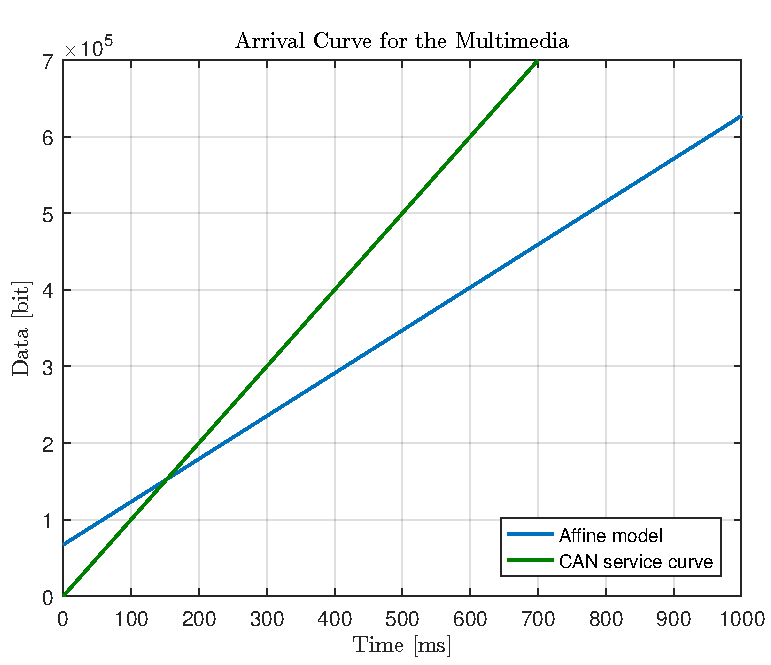
\includegraphics[width=.46\textwidth]{figures/ArrivalCurvesMultimedia}
	}
	\hspace{5pt}
	\captionbox
	{
		Arrival curves for the RC and service curve for the CAN-bus.
		\label{fig:ArrivalCurvesRC}
	}
	{
		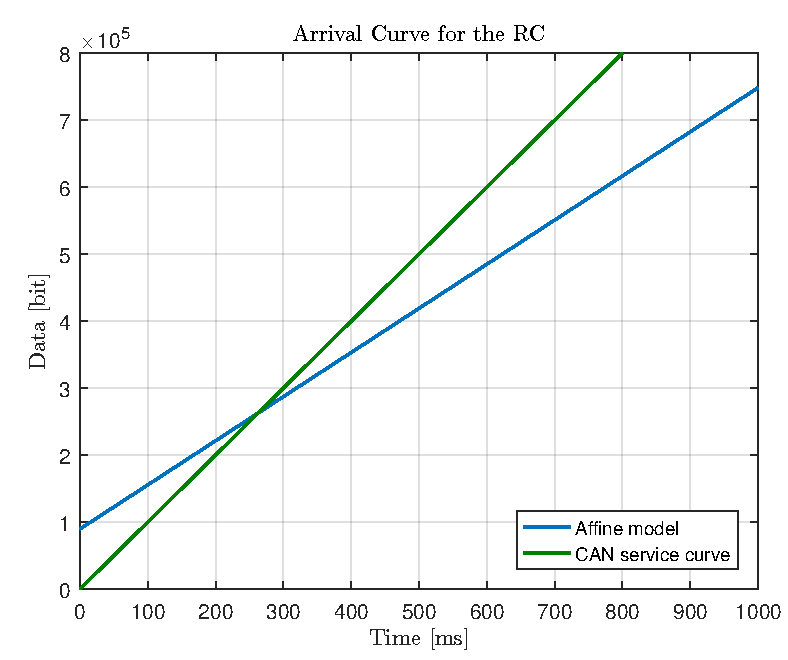
\includegraphics[width=.46\textwidth]{figures/ArrivalCurvesRC}
	}
\end{figure}

\subsection{Service Model}
The curve for the service model, $r(t)$, is seen in \autoref{fig:arrivalCurves}. The model is linear and defined by the capabilities of the CAN Bus with a rate of \SI{1}{Mbps}.